The python package plotly \cite{plotly} is used to display the network. Usually this 
package allows for the creation of figures which are then displayed in jupyter notebooks,
an extra window or saved as PNGs. However if only plotly is used there is no way to
edit a created figure without completely regenerating it which then opens a new window
that shows the figure. For this use case the figures must be able to update within the 
same window so the simulation and different settings for viewing the networks are possible.

To achieve this the figures plotly creates can be hosted on a webserver which is then
able to update the network that the website displays. Plotly offers a builtin website framework
called dash. The dash app is created using the statement in listing \ref{lst:dash_app}.
The CSS of the website uses the dash bootstrap CSS as a base and font awesome 
\cite{fontAwesome} is used for the icons. The assets folder is set because the website
uses some custom CSS located in that folder, that changes some of the default dash bootstrap CSS.

\begin{lstlisting}[language=python, caption={Instatiate a new Dash app}, label={lst:dash_app}]
app = Dash(
    external_stylesheets=[dbc.themes.BOOTSTRAP, dbc.icons.FONT_AWESOME],
    assets_folder=os.getcwd() + "/assets",
    suppress_callback_exceptions=True,
)
app.layout = dash.html.div(id="page-content")
app.run()
\end{lstlisting}

After calling \texttt{app.run()} this app automatically starts a flask server which hosts 
the website on \texttt{http://localhost:8050}. To specify what the website displays the
\texttt{layout} property of the \texttt{app} is set to the desired HTML components. For this
plotly offers HTML components as python classes as well as some custom bootstrap components
which are more advanced HTML elements like a sidebar. In this
case a simple div with the id \texttt{page-content} is used. The children of this div
are then changed according to which website needs to be displayed.

The webapp consists of three different pages:
\begin{itemize}
    \item \textbf{View}: Displays a 3D network and offers some controls to alter the appearance
    \item \textbf{Simulation}: Displays the same network as the view does with the same controls and
    offers functionality to run the simulation in that network.
    \item \textbf{Stats}: Shows stats collected during the simulation with controls for which 
    stats to display
\end{itemize}

For this three routes are created for the app so each website has its own URL: \texttt{/view},
\texttt{/sim} and \texttt{/stats}. To display the correct website for each URL a callback 
is used to change the content of the \texttt{page-content} div. This callback is called
whenever any URL of the webserver is accessed, it is shown in listing \ref{lst:page_content}.
\begin{lstlisting}[language=python, caption={Create callback for page content}, label={lst:page_content}]
@callback(
            Output("page-content", "children"),
            [Input("url", "pathname")],
)
def display_page(pathname):
    if pathname == "/view":
        html_view.reset()
        return html_view.layout
    elif pathname == "/sim":
        sim_view.reset()
        return sim_view.layout
    elif pathname == "/stats":
        stats_view.reset()
        return stats_view.layout
    else:  # if redirected to unknown link
        return "404"
\end{lstlisting}

\section{Network View}
The website for the network view consists of a collapsible sidebar on the left side which provides the
controls for the appearance of the network. The rest of the page is used to display the 
network. Figure \ref{fig:web_network_view} depicts the UI of this page.

\begin{figure}
    \centering
    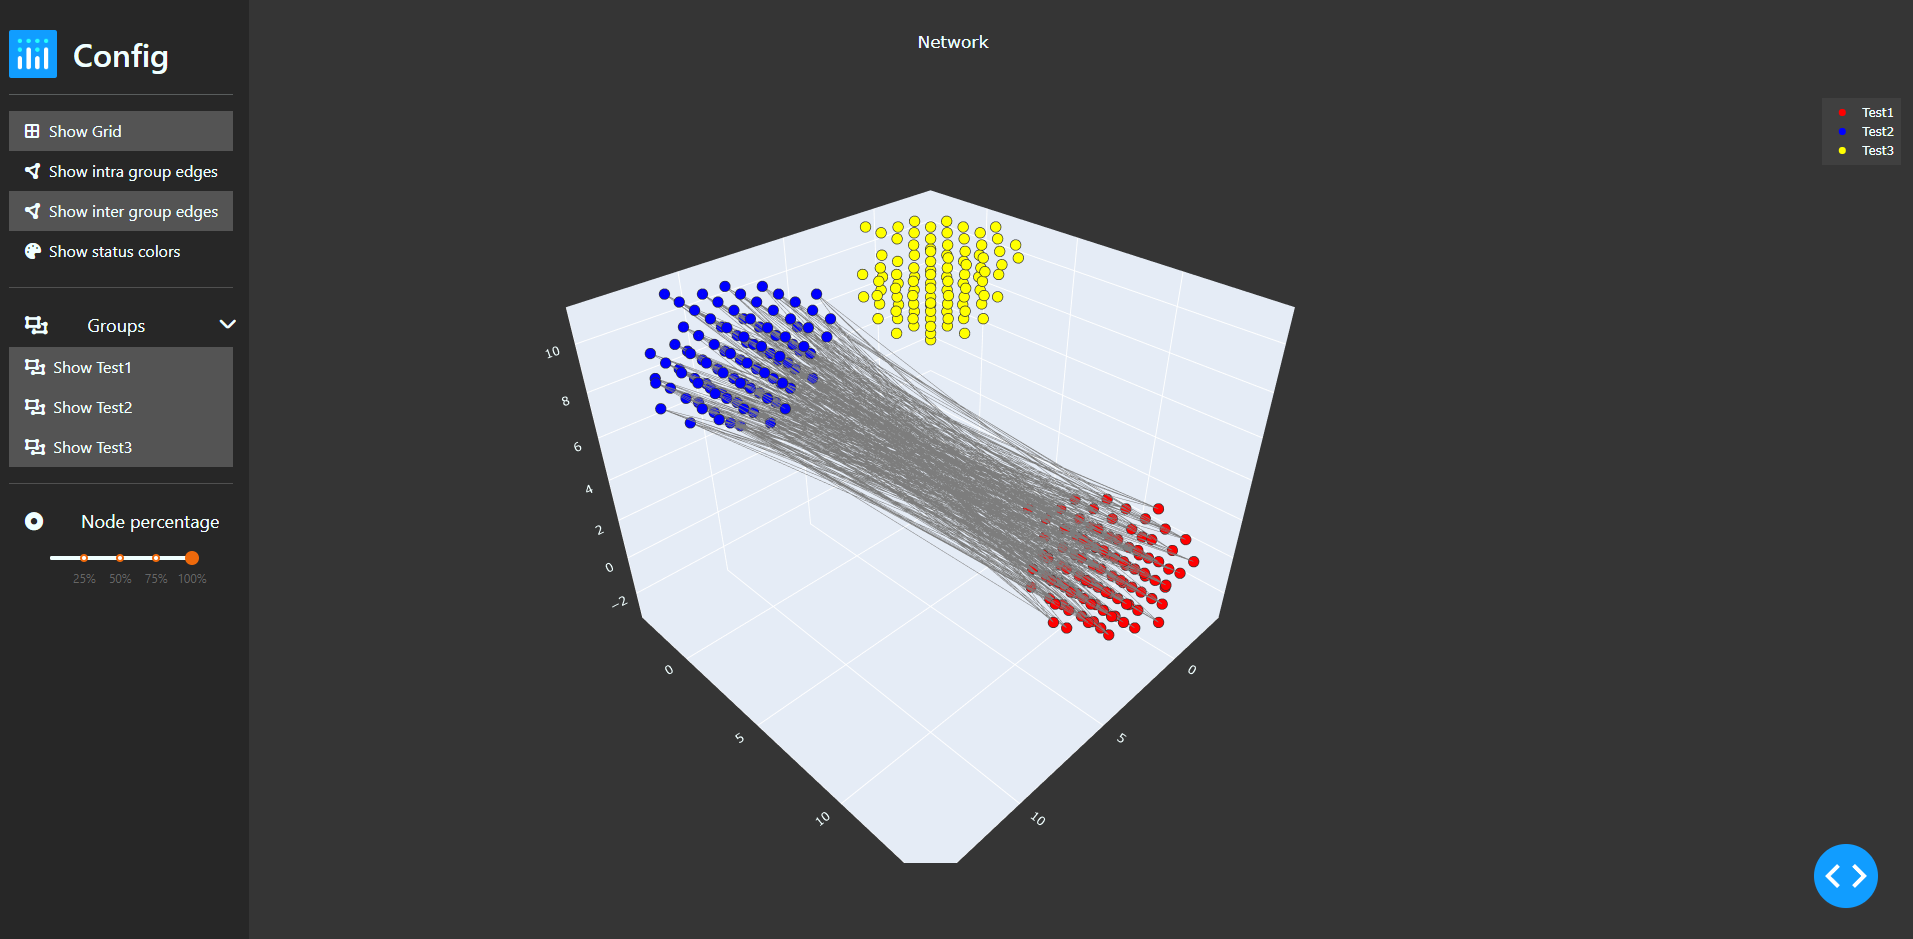
\includegraphics[width=0.5\linewidth]{images/web_network_view.png}
    \caption{UI for the network view webpage}
    \label{fig:web_network_view}
\end{figure}

The sidebar contains buttons to visually disable or enable the grid, intra/inter group edges, group/status color or 
groups of nodes. The slider can be used to reduce the amount of displayed nodes which 
can help to improve performance for large networks. Each of these settings uses a callback
to update the network. Listing \ref{lst:grid_callback} contains one such callback for toggling the grid. This
callback updates the style of the button to change the background color, depending on
whether the button is now activated or deactivated. The \texttt{update\_graph\_grid} edits
the required settings in the plotly figure to enable or disable the grid and then returns
the udpated figure. The two return values of the \texttt{toggle\_grid} function are passed
to the specified outputs which contain the ids of the UI elements for the button and network
figure. By using these outputs dash ensures the changes are represented on the website without
needing to reload it. Similar callbacks are created for the other buttons and the slider.

\begin{lstlisting}[language=python, caption={Callback for toggling the grid}, label={lst:grid_callback}]
@callback(
    [
        Output(self.id_factory("grid-button"), "style"),
        Output(self.id_factory("live-graph"), "figure", allow_duplicate=True),
    ],
    [Input(self.id_factory("grid-button"), "n_clicks")],
    prevent_initial_call=True,
)
def toggle_grid(_):
    self.sidebar.show_grid = not self.sidebar.show_grid
    return {
        "background-color": self.ENABLED_COLOR
        if self.sidebar.show_grid
        else self.BACKGROUND_COLOR
    }, self.update_graph_grid(self.sidebar.show_grid)
\end{lstlisting}

The plotly figure for the network which makes up the rest of the webpage offers some controls
to view the 3D network. The camera can be rotated by holding down the left mosue button
or moved by holding down the right mouse button. The zoom can be changed with the mouse wheel
and in the top right corner there are buttons for these controls as wells as a button to download
the current view as a png. Chapter \ref{cha:network_display} explains how the network figure
is created.

\section{Simulation view}
The simulation view contains the same UI as the network view. Its class inherits from the
network view. Then 5 new buttons to control the simulation are added: reset simulation,
show log outputs, advance one step, turn on auto advancing (1 step per second) and 
save stats. Using these five buttons as wells as the sidebar to control the appearance
of the network, the simulation can be run which will update the graph with new colors
for the current state of each node after each step. This is done in the callback of the
advance step button as shown in listing \ref{lst:step_callback} which runs one simulation
step and then creates the new color sequence and log output. The updated graph and log console
text are then returned to outputs to update the website.

\begin{lstlisting}[language=python, caption={Callback for advancing simulaton by one step}, label={lst:step_callback}]
@callback(
    Output(self.id_factory("live-graph"), "figure", allow_duplicate=True),
    Output("log-console-content", "children", allow_duplicate=True),
    Input(self.id_factory("step"), "n_clicks"),
    prevent_initial_call=True,
)
def step(_):
    with self.sim_mutex:
        self.sim.simulate_step()
        color_map, _ = self.sim.create_color_seq()
        if self.show_logs:
            return (
                self.graph.update_status_colors(color_map),
                self.sim.stats.get_log_text_html(),
            )
        else:
            return self.graph.update_status_colors(color_map), ""
\end{lstlisting}

The reset buttons opens a popup which requires confirmation of the user before the simulation
is actually reset. The save button also opens a popup which allows the user to enter a name
for the statistics of this simulation.

\section{Stats view}
The stats website displays statistics saved during simulations. When the website is first
opened a popup is shown where the user needs to select which statistics to display. This
website contains a similar sidebar as the previous view and simulation sites. The sidebar
contains buttons to control graphs of which statistics are displayed. The UI is depicted in figure
\ref{fig:web_stats_view}.

\begin{figure}
    \centering
    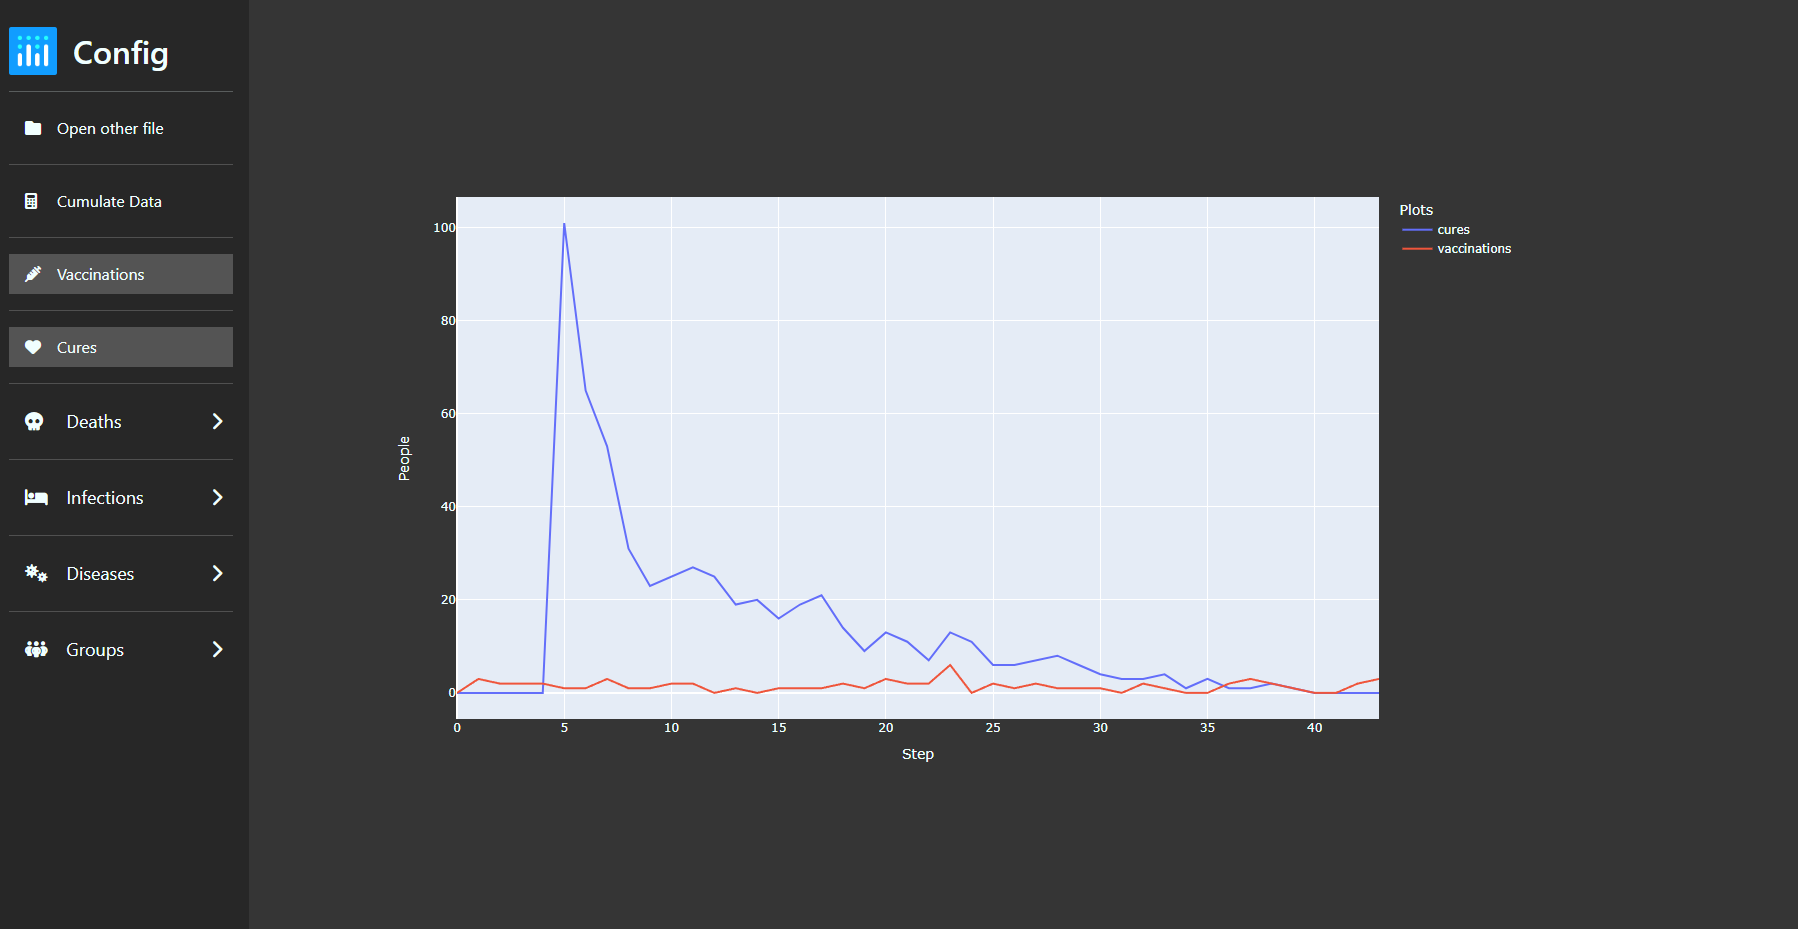
\includegraphics[width=0.5\linewidth]{images/web_stats_view.png}
    \caption{UI for the stats webpage}
    \label{fig:web_stats_view}
\end{figure}

The sidebar contains the following buttons:
\begin{itemize}
    \item Open another file: Brings the popup to select another stat file back up
    \item Cumulate data: Cumulates the graphs to show total up until each step instead of individual values of each step
    \item Display vaccinations, cures, deaths or infections data. Deaths and infections are split
    into total, vaccinated and unvaccinated
    \item Groups and diseases buttons allow to split the data to show only the values for a specific group/disease
    or the total for all diseases/groups
\end{itemize}
These buttons use callbacks to update the graphs similar to the ones for the network view.

\section{Updating the data}
To update the network or availabe stats files that are displayed endpoints are created.
The dash server allows the creation of listeners on URLs which are called if other
applications send HTML POST requests to those URLs. To update the data two endpoints
are exposed, one for updatig the network and one for updating the stat files.
The creation of these endpoints is shown in listing \ref{lst:data_endpoints}.
After a POST request is received the json data it contains is decoded and saved
for the stats or decoded, built and saved for networks. Then the view is reset to update
all open websites. At the end either a response for success (200) or failure (400) is sent.

\begin{lstlisting}[language=python, caption={Endpoints for updating data}, label={lst:data_endpoints}]
@app.server.route("/update-data", methods=["POST"])
def update():
    try:
        json_data = request.get_json()
        project.network = Network.from_dict(json_data)
        project.network.build()
        graph.update_network(project.network)
        html_view.reset()
        sim_view.reset()
        stats_view.reset()
        return make_response(jsonify({"status": "OK"}), 200)
    except Exception as e:
        return make_response(jsonify({"status": {str(e)}}), 400)

@app.server.route("/update-stats", methods=["POST"])
def update_stats():
    try:
        json_data = request.get_json()
        stats = SimStats.from_dict(json_data["stats"])
        project.stats[json_data["filename"]] = stats
        stats_view.reset()
        return make_response(jsonify({"status": "OK"}), 200)
    except Exception as e:
        return make_response(jsonify({"status": {str(e)}}), 400)
\end{lstlisting}
